\chapter{\term{ROCm} 函式庫 - 魏士勛}
\label{chap:ROCm 函式庫}
在 \chapref{chap:getting_started_with_hip_programming}、\chapref{chap:AMD_GPU_internal}、\chapref{chap:GPU_programming_patterns} 和 \chapref{chap:HIP_runtime_API} 集中於使用 \term{HIP} 程式語言為 AMD GPU 創建功能強大且高效的程式。在本章中,我們將介紹 \term{ROCm} 平台提供的常用官方函式庫。整合這些函式庫不僅可以節省寶貴的開發時間,還能幫助非專業使用者更快地發揮 GPU 的效能。

少數幾種算法和應用佔據了 GPU 執行的主要週期,其中最常見的是矩陣乘法運算,其次是線性代數計算。針對每個問題重新編寫這些操作會導致不必要的重複並浪費程式設計師的時間。因此,\term{HIP} 函式庫提供了經過配置管理的程式碼 reuse,既節省時間又減少除錯需求。

一般來說,GPU 程式設計比 CPU 程式設計更具挑戰性。例如,大量的 GPU kernel thread 需要程式設計師考慮 thread 的集體行為,而非一個部分的行為。同時,GPU 程式的高度併發性也使得除錯更加困難。因此,提升 GPU 程式效能需要對 GPU 硬體有深入的理解。非專業的 GPU 程式設計師在編寫和調整 GPU 程式時往往會遇到困難,即使是有經驗的程式設計師也難以從 GPU 中「榨取每一滴」效能。\term{HIP} 提供了針對常用算法高度優化的函式庫,以提高程式設計師的生產力。這些函式庫還可以在程式中直接調用,而無需關注實現細節。

本章介紹了一些廣泛使用的 \term{HIP} 函式庫,包括 \term{rocBLAS}、\term{rocSPARSE}、\term{rocFFT} 和 \term{rocRAND}。通常,對應於以「roc」為前綴的 \term{ROCm} 函式庫,每個函式庫都有一個以「hip」為前綴的 \term{HIP} 函式庫。\term{ROCm} 函式庫為 \term{ROCm} 平台提供高效能的實現,而 \term{HIP} 函式庫則作為一個輕量的相容層,分別在 AMD 或 NVIDIA GPU 平台上調用對應的 \term{ROCm} 或 \term{CUDA} 函式庫。本章將說明如何使用 \term{ROCm} 函式庫。讀者可以參考 \url{https://docs.amd.com/category/libraries}
,通過對程式碼進行少量修改來使用 \term{HIP} 函式庫。此外,讀者也可以通過上述連結找到更多函式庫的相關文檔。

\section{\term{rocBLAS}}
線性代數算法在平行 GPU 計算中受益良多。\term{HIP} 提供了 \term{rocBLAS} 函式庫,實現了最常用的線性代數算法。該函式庫遵循傳統基本線性代數子程式(\term{BLAS})函式庫的原則(這些函式庫最早於 1979 年以 Fortran 函式庫形式發布)。因此,程式設計師可以輕鬆找到 \term{BLAS} 與 \term{rocBLAS} API 之間的一對一對應關係。對於 GPU 程式設計師來說,\term{HIP} 的相容性帶來的一大優勢是他們可以利用現有的程式設計技能來開發與硬體無關的軟體產品。

\subsection{使用 \term{rocBLAS}}
\lstref{lst:rocBLAS} 示範了使用最簡單的 \term{rocBLAS} 函式之一:\term{rocblas\_sswap}。此函式僅需將緩衝區 dx 和 dy 中儲存的兩個向量內容互換。

\begin{lstlisting}[language=C, caption={\term{rocBLAS} 函式庫範例。為簡化起見,錯誤處理程式碼已省略。}, captionpos=t, label={lst:rocBLAS}]
#include <hip∕hip_runtime.h>
#include <rocblas.h>
#include <vector>

int main() {
    rocblas_int n = [vec_size]; ∕∕ Replace [vec_size] with an integer.
    float *dx, *dy;
    std::vector<float> hx(n);
    std::vector<float> hy(n);

    ∕∕ Initialize host memory. Omitted.

    ∕∕ Allocate device memory.
    hipMalloc(&dx, n * sizeof(float));
    hipMalloc(&dy, n * sizeof(float));

    ∕∕ Copy host memory to device.
    rocblas_set_vector(n, sizeof(float),
        hx.data(), 1, dx, 1);
    rocblas_set_vector(n, sizeof(float),
        hy.data(), 1, dy, 1);

    ∕∕ Create rocBLAS handle.
    rocblas_handle handle;
    rocblas_create_handle(&handle);

    ∕∕ Call the swap function. The "s" before "swap"
    ∕∕ indicates the function being called works with
    ∕∕ single-precision data.
    rocblas_sswap(handle, n, dx, 1, dy, 1);

    ∕∕ Copy the data back from the GPU memory.
    rocblas_get_vector(n, sizeof(float),
        dx, 1, hx.data(), 1);
    rocblas_get_vector(n, sizeof(float),
        dy, 1, hy.data(), 1);

    ∕∕ Release resources.
    hipFree(dx);
    hipFree(dy);
    rocblas_destroy_handle(handle);

    return 0;
}
\end{lstlisting}

儘管這個範例相對簡單,但仍有一些重點值得注意。

首先,使用 \term{rocBLAS} 函式庫的程式必須包含 \bold{rocblas.h} 標頭檔。在安裝了標準 \term{ROCm} 的系統中,該標頭檔可以在 \term{/opt/rocm/include} 或 \term{/opt/rocm/rocblas/include} 目錄中找到。此外,使用 \term{rocBLAS} 的程式也必須包含 \bold{hip/hip\_runtime.h} 標頭檔,因為程式仍然需要依賴常規的 \term{HIP} API 來正常運作。

其次,\term{rocBLAS} 運作於常規由 \term{HIP} 分配的 GPU 緩衝區上。對於記憶體管理,我們仍然依賴基本的 \term{HIP} API,例如 \term{hipMalloc} 和 \term{hipFree}。

第三,\term{rocBLAS} 提供了一組輔助函式,包括 \term{rocblas\_set\_vector}、\term{rocblas\_get\_vector}、\term{rocblas\_set\_matrix} 和 \term{rocblas\_get\_matrix},用於在 CPU 和 GPU 之間傳輸數據。此外,\term{rocblas\_set\_vector} 和 \term{rocblas\_get\_vector} 函式需要兩個額外的整數參數。在 \lstref{lst:rocBLAS} 中,我們始終將這些參數賦值為 1,因為它們用於描述儲存數據的記憶體佈局。具體而言,這兩個函式中的參數表示需要複製的數據結構的 stride。如果將第 18 和 19 行按照 \lstref{lst:different} 的方式重寫,輔助函式將從 hx 向量中每隔一個值複製一次,並將這些值緊密地放置在 dx 向量中。

\begin{lstlisting}[language=C, caption={使用不同值的範例。}, captionpos=t, label={lst:different}]
∕∕ This line is equivalent to the following.
∕∕ dx[0] = hx[0];
∕∕ dx[1] = hx[2];
∕∕ dx[2] = hx[4];
∕∕ ...
rocblas_set_vector(n, sizeof(float),
    hx.data(), 2, dx, 1);
\end{lstlisting}

第四,儘管我們在 \lstref{lst:rocBLAS} 中省略了錯誤處理代碼,但在實際產品中使用 \term{rocBLAS} 的程式應該妥善處理錯誤。大多數 \term{rocBLAS} 函式會返回一個 \bold{rocblas\_status} 狀態碼,因此程式需要檢查返回值是否為 \bold{rocblas\_status\_success}。其他返回值則表示執行不正常,因此應仔細檢查錯誤代碼。\lstref{lst:APIerror} 展示了一個處理 \term{rocBLAS} 錯誤的簡單範例。

\begin{lstlisting}[language=C, caption={處理 \term{rocBLAS} API 錯誤的範例。}, captionpos=t, label={lst:APIerror}]
rocblas_status status;
status = rocblas_set_vector(n, sizeof(float),
    hx.data(), 1, dx, 1);
if (status != rocblas_status_success) {
    printf("Failed to set vector.\n");
    exit(-1);
}
\end{lstlisting}

第五,在調用大多數 \term{rocBLAS} 函式時,需要一個 handle,因為它用於儲存多個 \term{rocBLAS} 函式調用之間共享的上下文資訊。除了簡單的輔助函式之外,必須在調用函式之前創建 handle,這一過程如 \lstref{lst:rocBLAS} 的第 25 行所示。在使用完 \term{rocBLAS} 函式後,必須釋放 handle 以釋放佔用的資源。

最後,如 \lstref{lst:rocBLAS} 的第 30 行所示,我們必須調用 \term{rocBLAS} 函式來執行線性代數操作。該函式庫提供了廣泛的線性代數函式,我們會在 \secref{sec:rocBLAS_function} 中進一步介紹。

\subsection{\term{rocBLAS} 函式} \label{sec:rocBLAS_function}
\term{rocBLAS} 函式分為三個層級。第一層包含執行向量與向量操作的函式。第二層和第三層分別提供矩陣與向量操作,以及矩陣與矩陣操作的函式。

不同的 \term{rocBLAS} 函式包括設計用於不同數據類型的變體,可以從函式名稱中推斷其作用。一般來說,\term{rocBLAS} 函式的命名格式為 \bold{rocblas\_[type][operation]}。例如,在 \bold{rocblas\_sswap} 中,\bold{s} 表示數據類型,而 swap 表示操作名稱。支援的數據類型完整列表請參見 \tabref{tab:rocblas_data_types}。

\begin{table}[h!]
    \centering
    \caption{rocBLAS 支援的數據類型。}
    \label{tab:rocblas_data_types}
    \begin{tabular}{cl}
        \hline
        \textbf{Letter} & \textbf{Data Type} \\ \hline
        s & Single-Precision Floating-Point Numbers \\ 
        d & Double-Precision Floating-Point Numbers \\ 
        h & Half-Precision Floating-Point Numbers (16 bits per number) \\ 
        b & 16-bit Brain Floating-Point Number [40] \\ 
        c & Single-Precision Complex Numbers (both real and imaginary parts are single-precision) \\
        z & Double-Precision Complex Numbers (both real and imaginary parts are double-precision floating-point numbers) \\ \hline
    \end{tabular}
\end{table}

\term{rocBLAS} 還支援 batch 和 strided-batch。batched 線性代數透過單一函式呼叫處理多個輸入元素。Batch 函式在 \term{rocBLAS} 函式名稱中以 \bold{\_batched} 為後綴。例如,\term{rocblas\_sdot\_batched} 是常規函式 \term{rocblas\_sdot} 的 batch 版本,用於計算多組向量對的點積。其輸出是一個向量,而非常規版本函式的標量值。

Strided-batch 允許函式僅對輸入 batch 中的部分元素執行操作。例如,若 batch 大小為 5,且 stride 為 2,則函式將處理輸入陣列中的第 0、2 和 4 個元素。這類操作在 \term{rocBLAS} 函式名稱中會加上 \texttt{"strided\_batched"} 後綴。

\subsection{非同步執行}
前面我們提到,GPU kernel 在執行過程中以 CUDA 流的形式啟動,\term{rocBLAS} kernel 也不例外。預設情況下,\term{rocBLAS} kernel 是以非同步的方式啟動到預設的 NULL CUDA 流。因此,程式設計師不應假設函式返回後結果會立即準備就緒。相反,需要使用 \term{HIP} API(例如 \term{hipDeviceSynchronize} 或 \term{hipStreamSynchronize})進行適當的同步操作。使用預設非同步執行模型的優勢在於其程式設計的簡單性,這種模型允許將 CPU 執行與 \term{rocBLAS} 操作同時進行(請參見 \lstref{lst:overlap})。

\begin{lstlisting}[language=C, caption={\term{rocBLAS} 與 CPU 同時執行。}, captionpos=t, label={lst:overlap}]
rocblas_sgemm(arguments...);
∕∕ CPU work that overlaps with the rocblas_sgemm call.
hipDeviceSynchronize();
\end{lstlisting}

也可以使用 CUDA 流來控制同時呼叫的 API 。通過 \term{rocBLAS} API 呼叫,handle 會追蹤所使用的 CUDA 流。值得注意的是,使用多個 CUDA 流可以讓執行階段、驅動程式和硬體控制同時執行。如 \lstref{lst:stream} 所示,如果 GPU 擁有足夠的資源,第 10 行和第 13 行的 API 呼叫(例如 \bold{rocblas\_sgemm})可以同時執行。

\begin{lstlisting}[language=C, caption={多 device 與多 CUDA 流的 \term{rocBLAS} 執行}, captionpos=t, label={lst:stream}]
hipStream_t stream1, stream2;
rocblas_handle handle;

hipStreamCreate(&stream1);
hipStreamCreate(&stream2);

rocblas_create_handle(&handle);

rocblas_set_stream(stream1);
∕∕ API call 1 that uses stream1

rocblas_set_stream(stream2);
∕∕ API call 2 that uses stream2

hipStreamSynchronize(stream1);
hipStreamSynchronize(stream2);

∕∕ Destroy the streams and the handle.
\end{lstlisting}

\subsection{MI100 上的 \term{rocBLAS}}
CDNA/CDNA2 GPU 配備了矩陣運算單元,可大幅加速矩陣乘法計算。\term{rocBLAS} 的實現會在可能的情況下自動使用矩陣運算單元,無需顯式開啟或關閉這些單元。

\begin{figure}
    \centering
    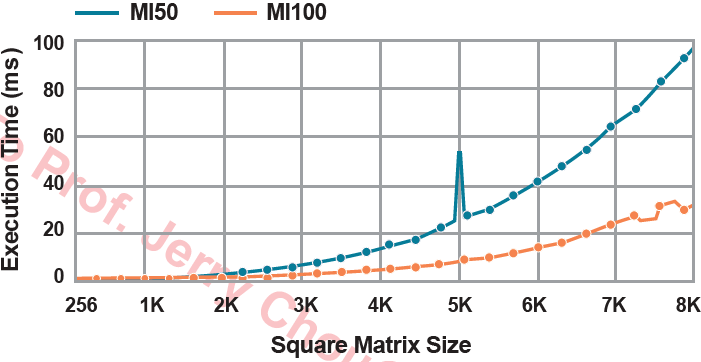
\includegraphics[width=0.9\linewidth]{FileAusiliari/Screenshots/Figure9-1.png}
    \caption{MI100 與 MI50 的效能比較。嘗試使用 MI200。}
    \label{fig:MI100}
\end{figure}

為了了解矩陣運算單元帶來的效能提升,我們在 MI100 和 MI50 GPU 上運行了 \term{rocBLAS} 的單精度通用矩陣乘法(SGEMM)API(見 \figref{fig:MI100})。以兩個大小為 8,192×8,192 的矩陣相乘為例,理論上所需的運算次數為 2 × 8,192 × 8,192 × 8,192 ≈ 1.1T。
MI50 GPU 在 95.7 毫秒內完成計算,達到 10.45 TFLOPS 的有效計算吞吐量,而其理論吞吐量為 13.41 TFLOPS。因此,MI50 GPU 已經達到了極高的效能利用率(81\%)。然而,MI100 GPU 的速度快了 3.14 倍,僅用 30.4 毫秒完成相同的矩陣運算。在 MI100 上執行可實現 32.84 TFLOPS 的有效吞吐量,相當於理論計算吞吐量的 149\%(如果僅考慮 SIMD 單元的執行)。這種看似不可能的高效能利用率,只有在使用矩陣運算單元時才能實現。
由此我們可以清楚地看到,使用矩陣運算單元顯著提升了線性代數操作的整體效能。

\subsection{從舊版的 \term{BLAS} 函式庫移植}
從高層次來看,傳統 \term{BLAS} 函式庫的 API 與 \term{rocBLAS} API 之間具有一對一的對應關係。這種對應相對簡單,因為 API 名稱基本保持不變,唯一的區別是 \term{rocBLAS} 使用小寫的 API 名稱,並以 \term{rocblas\_} 作為前綴。此外,參數列表需要進行少量修改。\term{rocBLAS} API 要求每個函式的第一個參數是 \bold{rocblas\_handle}。如果舊版的 API 返回一個值,則該值必須作為最後一個參數傳入,供 \term{rocBLAS} API 返回 \bold{rocblas\_status}。

為了保持 \term{rocBLAS} 與舊版 \term{BLAS} API 的一致性,\term{rocBLAS} 假設矩陣是以 1 為基準(即索引從 1 開始而非 0)且為列優先存儲。然而,這與 \term{C} 程式設計的慣例不同,後者的矩陣索引通常是以 0 為基準且為行優先存儲。因此,處理用 \term{C/C++} 創建的矩陣時需特別小心。

\section{\term{rocSPARSE}}
現實世界中的數據通常是稀疏的,大部分值為零。例如,若使用矩陣來表示 Facebook 用戶的好友關係,大多數元素將為空,因為大多數用戶之間並非好友。矩陣中零值所占的百分比稱為「sparsity」。Sparsity 為 90\%(密度為 10\%)表示矩陣中 90\% 的元素為零。由於稀疏矩陣被廣泛用於表示現實數據,高效的處理至關重要。稀疏矩陣的特殊性表明,不應使用密集矩陣的算法來處理它們。

使用 \term{rocBLAS} 提供的常規方法執行稀疏線性代數操作(例如通用矩陣乘法(GEMM))在記憶體管理和計算方面可能效率低下。將稀疏矩陣存儲為密集矩陣會浪費大量記憶體,因此需要壓縮存儲。典型的 GPU 僅能執行每軸包含數萬個元素的密集 GEMM 操作,但現實中的稀疏數據集每軸可能包含數百萬個元素。如果將這些數據以密集格式存儲,GPU 記憶體將很快被填滿。此外,對零值進行計算是浪費的,因為結果總是零。更糟的是,GPU 記憶體層次結構會不斷將大量零值傳輸到 computing core,浪費記憶體頻寬和快取空間。

\term{rocSPARSE} 和 \term{rocBLAS} 函式庫提供了基於稀疏向量和矩陣的高效線性代數計算。這兩個函式庫最初為 CPU 開發。本節將介紹稀疏數據的表示方法,隨後討論 \term{rocSPARSE} 支援的線性代數計算。

\subsection{稀疏數據表示法}
稀疏矩陣有多種表示方法,每種方法根據不同的使用場景各有優缺點。通常,這些方法通過標量值和向量記錄矩陣的內容,包含原始矩陣的所有資訊(即無損壓縮)。因此,可以從稀疏表示轉換回密集表示。在此,我們介紹幾種常用的稀疏數據表示方法。

座標格式(COO) 表示法記錄非零值及其座標。一個 COO 矩陣需要三個標量數據:\bold{m}(行數)、\bold{n}(列數)、\bold{nnz}(非零元素的數量)。矩陣的內容存儲為三個向量:第一個向量 \bold{coo\_val} 包含所有非零值,按照其行和列索引排序。對於每個非零值,其 x 和 y 座標分別存儲在 \bold{coo\_col\_ind} 和 \bold{coo\_row\_ind} 向量中。

例如,矩陣:

\[
A = \begin{pmatrix} \tag{9.1}
1.0 & 2.0 & 0.0 & 3.0 & 0.0 \\
0.0 & 4.0 & 5.0 & 0.0 & 0.0 \\
6.0 & 0.0 & 0.0 & 7.0 & 8.0
\end{pmatrix}
\]

應被改寫為

\[
\begin{aligned} 
m &= 3, \; n = 5, \; nnz = 8 \\
\text{coo\_val} &= [1.0, 2.0, 3.0, 4.0, 5.0, 6.0, 7.0, 8.0] \\
\text{coo\_row\_ind} &= [0, 0, 0, 1, 1, 2, 2, 2] \\
\text{coo\_col\_ind} &= [0, 1, 3, 1, 2, 0, 3, 4]
\end{aligned} \tag{9.2}
\]

壓縮稀疏列(CSR)在多種情境中非常高效,儘管 COO 因其簡單性通常更具優勢。然而,COO 需要大約 3×\term{nnz} 的存儲空間,這可能不足夠高效。

與 COO 類似,CSR 需要相同的三個標量值、相同的非零向量和相同的列索引向量。唯一的區別在於行索引向量。

在 CSR 中,使用 \bold{csr\_row\_ptr} 向量記錄 \bold{csr\_val} 向量中每行第一個元素的偏移量。\bold{csr\_row\_ptr} 向量的第一個元素必須是 0,因為它也是 \bold{csr\_val} 的第一個元素。如果矩陣的第一行有三個非零元素,則 \bold{csr\_row\_ptr} 向量的第二個元素將是 3,因為第二行的第一個元素在 \bold{csr\_val} 中的索引為 3。如果某行中沒有非零元素,我們仍需要將該行的行號添加到 \bold{csr\_row\_ptr} 中。在這種情況下,其值將是 \bold{csr\_row\_ptr} 中下一個數字的索引。

使用與上述相同的例子,我們應該將矩陣改寫為:

\[
A = \begin{pmatrix} \tag{9.3}
1.0 & 2.0 & 0.0 & 3.0 & 0.0 \\
0.0 & 4.0 & 5.0 & 0.0 & 0.0 \\
0.0 & 0.0 & 0.0 & 0.0 & 0.0 \\
6.0 & 0.0 & 0.0 & 7.0 & 8.0
\end{pmatrix}
\]

使用 CSR 表示法

\[
\begin{aligned} 
m &= 4, \; n = 5, \; nnz = 8 \\
\text{csr\_val} &= [1.0, 2.0, 3.0, 4.0, 5.0, 6.0, 7.0, 8.0] \\
\text{csr\_row\_ptr} &= [0, 3, 3, 5, 8] \\
\text{csr\_col\_ind} &= [0, 1, 3, 1, 2, 0, 3, 4]
\end{aligned} \tag{9.4}
\]

CSR 格式適用於逐行處理。以上述範例為例,若一個執行緒需要處理第 1 行,該執行緒首先查找 \bold{csr\_row\_ptr} 向量中索引 1(值為 3)和索引 2(值為 5)。第 1 行中的非零元素數量可以通過索引 2 減去索引 1(5 − 3 = 2)輕鬆計算得出。為了使此過程適用於所有行(最後一行是特殊情況),需要在 \bold{csr\_row\_ptr} 的末尾添加 \bold{nnz} 作為額外的元素。因此,上述範例中的矩陣 \bold{A} 有 4 行,但 \bold{csr\_row\_ptr} 包含了 5 個數字。此外,\bold{csr\_row\_ptr} 中的索引 1 還用作 \bold{csr\_val} 和 \bold{csr\_col\_ind} 中的偏移量,用於定位元素的值和列索引。

CSR 的存儲需求大約為 2×\term{nnz}+\term{m},這比 COO 的 3×\term{nnz} 的存儲需求更高效(當 \term{m}<\term{nnz} 時)。對於大多數「非極稀疏」的矩陣,此條件成立。然而,在極度稀疏的情況下,COO 更高效。

\term{rocSPARSE} 函式庫還支援其他不常用的稀疏表示法。對此感興趣的讀者可參閱官方的 \term{rocSPARSE} 文檔以了解詳情。

\subsection{rocSPARSE 函式}
與 \term{rocBLAS} 類似,\term{rocSPARSE} 的函式也分為三個層級。第一層(Level 1) 的函式描述稀疏向量與密集向量之間的操作。第二層(Level 2) 描述稀疏矩陣與密集向量之間的計算。最後,第三層(Level 3) 描述稀疏矩陣與密集矩陣之間的計算。此外,\term{rocSPARSE} 支援四種數據類型(即單精度、雙精度、單精度複數和雙精度複數),分別以 \bold{s}、\bold{d}、\bold{c} 和 \bold{z} 為前綴表示。

\begin{lstlisting}[language=C, caption={使用 \term{rocSPARSE} 進行矩陣乘法的範例。一個矩陣以 CSR 格式表示,另一個矩陣以密集矩陣表示。為簡化起見,錯誤處理和記憶體釋放的程式碼已被省略。}, captionpos=t, label={lst:CSR}]
rocsparse_handle handle;
rocsparse_mat_descr descr;
float alpha, beta;
float *dVal;
int *dRowPtr, *dColInd;

rocsparse_create_handle(&handle)
rocsparse_create_mat_descr(&descr);

alpha = 1.0;
beta = 0.0;

∕∕ Allocate and fill in dVal, dRowPtr, dColInd.

rocsparse_scsrmm(
    handle,
    rocsparse_operation_none,
    rocsparse_operation_transpose,
    size, size, size,
    nnz, &alpha, descr, dVal, dRowPtr, dColInd,
    dB, size,
    &beta, dC, size);
hipDeviceSynchronize()
\end{lstlisting}

我們在 \lstref{lst:CSR} 中提供了一個使用 \term{rocSPARSE} API 的範例。與 \term{rocBLAS} 類似,\term{rocSPARSE} 需要一個 handle 物件來追蹤執行上下文。需要注意的是,\term{rocSPARSE} 的 handle 與 \term{rocBLAS} 的 handle 不同,當需要同時調用這兩個函式庫時,這些 handle 無法混用。每個 handle 僅適用於一個 device。因此,使用多個 device(即使非平行)時,需要為每個 device 創建一個 handle。此外,還需要一個 descriptor(\bold{descr},範例中於 \lstref{lst:CSR} 第 2 行宣告)來告知 API 關於稀疏矩陣的組織方式(例如,索引是以零為基準還是一為基準,矩陣是列優先還是行優先)。預設情況下,描述子被設置為零基且行優先,因此在我們的範例中無需進行更改。

\begin{figure}[h]
    \centering
    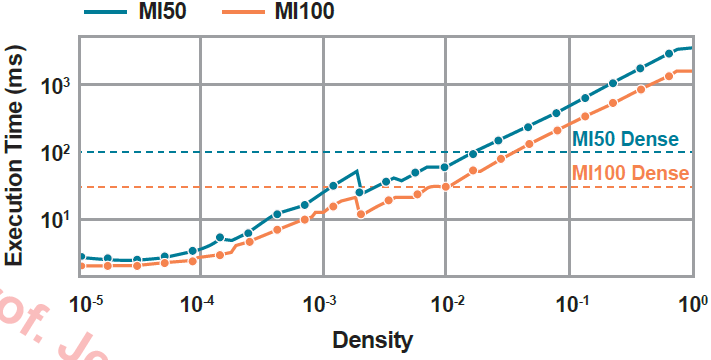
\includegraphics[width=0.9\linewidth]{FileAusiliari/Screenshots/Figure9-2.png}
    \caption{使用 \term{rocSPARSE} 的效能優勢。本範例使用 CSR 格式表示稀疏矩陣。如果使用其他格式,結果可能會有所不同。}
    \label{fig:CSR}
\end{figure}

選擇使用 \term{rocBLAS} 或 \term{rocSPARSE} 取決於問題的特性和底層硬體。通常,\term{rocSPARSE} 在高度稀疏的矩陣上表現優於 \term{rocBLAS}。為了說明兩者的比較,我們使用 \term{rocBLAS} 和 \term{rocSPARSE} 對兩個大小為 8,192 × 8,192 的矩陣進行乘法運算(參見 \figref{fig:CSR})。我們改變第一個矩陣的密度,觀察其對效能的影響。由於 \term{rocBLAS} 的效能與數據無關,因此可以將其效能視為水平線。在 \figref{fig:CSR} 中可以看到,隨著密度降低,\term{rocSPARSE} 的執行時間也隨之減少,因為矩陣中的非零元素更少,實際的計算和數據移動也減少。當密度低於 1\% 時,這一趨勢才會趨於平緩。比較密集和稀疏矩陣乘法的效能,我們可以觀察到,當密度分別低於 5\% 和 1\% 時,在 MI50 和 MI100 GPU 上,\term{rocSPARSE} 的表現優於 \term{rocBLAS}。

\section{\term{rocFFT}}
離散傅立葉變換(DFT)是一種常見的數位訊號處理操作,用於將訊號從 time domain 轉換到 frequency domain。DFT 將訊號分解為不同頻率下的振幅與相位。分解後的形式有助於分析濾波器或處理系統如何在不同頻率下改變訊號。此外,DFT 通常是卷積操作的第一步,而卷積是卷積神經網路(CNN)的核心部分。在 time domain 中的卷積相當於 frequency domain 中的乘法,而乘法的計算複雜度遠低於卷積。

一個典型的 DFT 公式如 \eqref{eq:DFT} 所示,其中 \term{x} 是輸入數據, $\tilde{x}$是輸出數據,符號 ± 表示轉換方向,+ 和 − 分別代表從 time domain 到 frequency domain 或從 frequency domain 到 time domain 的轉換方向。DFT 操作可以擴展到 2D 和 3D 數據,對應的公式分別如 \eqref{eq:DFT-2} 和 \eqref{eq:DFT-3} 所示。這些公式表明,直接 DFT 演算法的計算複雜度為 $O(N^2)$。外層迴圈計算每個輸出元素,內層迴圈則遍歷所有數據。

\begin{equation} \tag{9.5} \label{eq:DFT}
\tilde{x}_j = \sum_{k=0}^{n-1} x_k \exp\left(\pm i \frac{2\pi jk}{n}\right) \quad \text{for } j = 0, 1, \dots, n-1,
\end{equation}

\begin{align} \tag{9.6} \label{eq:DFT-2}
\tilde{x}_{jk} = \sum_{q=0}^{m-1} \sum_{r=0}^{n-1} x_{qr} 
\exp\left(\pm i \frac{2\pi jr}{n}\right) 
\exp\left(\pm i \frac{2\pi kq}{m}\right) \\
\text{for } j = 0, 1, \dots, n-1 \text{ and } k = 0, 1, \dots, m-1,
\end{align}

\begin{align} \tag{9.7} \label{eq:DFT-3}
\tilde{x}_{jkl} = &
\sum_{s=0}^{p-1} \sum_{q=0}^{m-1} \sum_{r=0}^{n-1} x_{rqs} 
\exp\left(\pm i \frac{2\pi jr}{n}\right) \exp\left(\pm i \frac{2\pi kq}{m}\right)  \exp\left(\pm i \frac{2\pi ls}{p}\right), \\
& \text{for } j = 0, 1, \dots, n-1 \\ 
& \text{and } k = 0, 1, \dots, m-1 \\ 
& \text{and } l = 0, 1, \dots, p-1.
\end{align}

快速傅立葉變換(FFT)本身並不是一種具體的演算法,而是一組演算法的總稱,用於以 $O(NlogN)$ 的複雜度執行 DFT 操作,這遠比直接 DFT 方法的 $O(N^2)$ 複雜度簡單得多。FFT 的演算法細節超出了本書的範疇,但需要注意的是,所有 FFT 演算法的輸出與直接 DFT 演算法的輸出完全相同。\term{rocFFT} 函式隱藏了這些細節,為程式設計師提供了一個簡單的介面,用於高效執行 DFT 操作。

\subsection{\term{rocFFT} 工作流程}
在 \lstref{lst:rocFFT} 中,使用 \term{rocFFT} 進行訊號處理需要遵循以下步驟:

首先,必須調用 \term{rocfft\_setup} 函式來初始化函式庫,而在程式結束時,必須調用 \term{rocfft\_cleanup} 函式以對應 \term{rocfft\_setup},進行資源清理。

接著,需要建立一個 FFT 執行計畫,該計畫描述執行操作的數據維度、佈局和類型(例如實數、複數、單精度或雙精度)。完成 FFT 操作後,必須銷毀該計畫以釋放相關資源。

隨後,外部需提供 FFT 演算法所需的緩衝區,並可通過 \term{rocfft\_plan\_get\_work\_buffer\_size} 函式來檢索緩衝區大小,該緩衝區需使用 \term{hipMalloc} API 分配,並通過 \term{rocfft\_execution\_info\_set\_work\_buffer} API 進行配置。

最後,通過調用 \term{rocfft\_execute} 函式執行操作。與其他調用 GPU kernel 的函式類似,\term{rocfft\_execute} 是非同步執行的,並在操作完成之前返回。因此,在檢索結果之前,需通過 \term{hipDeviceSynchronize} 函式進行同步。

\begin{lstlisting}[language=C, caption={使用 \term{rocFFT} 函式庫的範例。}, captionpos=t, label={lst:rocFFT}]
rocfft_setup();

size_t N = 16;
size_t Nbytes = N * sizeof(float2);

∕∕ Create \textit{HIP} device buffer
float2 *x;
hipMalloc(&x, Nbytes);

∕∕ Initialize data
std::vector<float2> cx(N);
for (size_t i = 0; i < N; i++) {
    cx[i].x = 1;
    cx[i].y = -1;
}

∕∕ Copy data to device
hipMemcpy(x, cx.data(), Nbytes, hipMemcpyHostToDevice);

∕∕ Create rocFFT plan
rocfft_plan plan = nullptr;
size_t length = N;
rocfft_plan_create(&plan,
    rocfft_placement_inplace,
    rocfft_transform_type_complex_forward,
    rocfft_precision_single,
    1, &length, 1, nullptr);

∕∕ Check if the plan requires a work buffer
size_t work_buf_size = 0;
rocfft_plan_get_work_buffer_size(plan, &work_buf_size);
void* work_buf = nullptr;
rocfft_execution_info info = nullptr;
if(work_buf_size) {
    rocfft_execution_info_create(&info);
    hipMalloc(&work_buf, work_buf_size);
    rocfft_execution_info_set_work_buffer(info, work_buf, work_buf_size);
}

∕∕ Execute plan
rocfft_execute(plan, (void**) &x, nullptr, info);

∕∕ Wait for execution to finish
hipDeviceSynchronize();

∕∕ Clean up work buffer
if(work_buf_size) {
    hipFree(work_buf);
    rocfft_execution_info_destroy(info);
}


∕∕ Use the results (skipped).

∕∕ Clean up
rocfft_plan_destroy(plan);
rocfft_cleanup();
\end{lstlisting}

\subsection{FFT 執行計畫}
從上述範例中可以看到,FFT 執行計畫是使用 \term{rocFFT} 函式庫的關鍵,因為它提供了關於待執行操作的詳細資訊。因此,我們需要說明如何建立 FFT 計畫。

在大多數情況下,FFT 計畫的建立是通過調用 \term{rocfft\_plan\_create} API 完成的。第一個參數是指向計畫的指標。第二個參數描述結果的存放位置,可以是 \bold{inplace}(即執行的輸出覆蓋輸入緩衝區)或 \bold{notinplace}(輸出存放在另一個 buffer 中)。第三個參數 \bold{transform\_type} 指定 FFT 是正變換(即從 time domain 到 frequency domain)還是反變換(即從 frequency domain  到 time domain),並說明數據是實數還是複數。這裡支持所有四種變換類型及其對應的數據類型組合。第四個參數是數據的浮點精度級別(例如,單精度或雙精度)。

上述的四個參數描述了 FFT 操作,而其他參數則用於描述數據。接下來的兩個參數代表數據的形狀,第五個參數描述數據的維度數量(1、2 或 3 維),第六個參數描述每個維度的大小。FFT 操作的輸入和輸出數據大小始終相同,因此只需一組大小參數即可描述輸入和輸出數據。\term{number\_of\_transforms} 參數允許通過一次調用 \term{rocfft\_execution} API 對多組數據應用相同的 FFT 轉換(即 batch)。最後,description 參數通常設置為 NULL,除非需要指定不尋常的數據佈局。

\begin{lstlisting}[language=C, caption={\term{rocfft\_plan\_create} 函式的部署。}, captionpos=t, label={lst:Signature}]
rocfft_status rocfft_plan_create(
    rocfft_plan *plan,
    rocfft_result_placement placement,
    rocfft_transform_type transform_type,
    rocfft_precision precision,
    size_t dimensions,
    const size_t *lengths,
    size_t number_of_transforms,
    const rocfft_plan_description description
)
\end{lstlisting}

\section{\term{rocRAND}}
隨機數生成對於許多高效能計算(HPC)應用來說是至關重要的。隨機數被用來避免確定性和可預測的結果,因此廣泛應用於加密、身份識別和隱私保護等功能。這也是蒙地卡羅模擬中的基礎步驟,因為它們用來研究隨機變量對特定系統的影響。

\term{rocRAND} 函式庫提供了高效的大量隨機數生成能力。\lstref{lst:rocRAND} 展示了使用 \term{rocRAND} 的範例。首先創建一個 \term{rocRAND} 隨機數生成器,接著設置種子,最後調用隨機數生成函式完成生成操作。

\begin{lstlisting}[language=C, caption={一個生成 100 萬個偽隨機數的 \term{rocRAND} 函式。}, captionpos=t, label={lst:rocRAND}]
#include <hip∕hip_runtime.h>
#include <rocrand.h>
#include <stdio.h>
#include <time.h>

int main() {
    size_t n = 1048576;

    rocrand_generator gen;
    float *d_rand;

    hipMalloc((void **)&d_rand, n * sizeof(float));

    ∕∕ Step 1: Create a random number generator.
    rocrand_create_generator(&gen, ROCRAND_RNG_PSEUDO_DEFAULT);

    ∕∕ Step 2: Set a seed.
    rocrand_set_seed(gen, time(NULL));

    ∕∕ Step 3: Generate the random numbers.
    rocrand_generate_uniform(gen, d_rand, n);

    ∕∕ Use the generated random numbers.

    rocrand_destroy_generator(gen);
    hipFree(d_rand);
    return 0;
}
\end{lstlisting}

\term{rocrand\_generate\_uniform} 是 \term{rocRAND} 提供的最簡單隨機數生成函式之一。程式設計師可以根據所涉及的數據類型調用不同的函式。\term{rocRAND} 支援生成以下數據類型的隨機數:chars(8 位無符號整數)、shorts(16 位無符號整數)、32 位無符號整數、半精度浮點數、單精度浮點數和雙精度浮點數。此外,該函式還支援根據不同分佈生成隨機數,包括均勻分佈、常態分佈、對數正態分佈和泊松分佈。分佈與數據類型的對應關係列於 \tabref{tab:rocRAND}。

這些 API 生成的是 pseudo-random 變數,每一個新生成的數都是獨立於上一個數生成的。因此,某些生成的數字可能在數值上非常接近上一個數。對於模擬來說,數值上接近的隨機數可能是不理想的,因為實驗通常需要多樣化或隨機的結果。在某些情況下,參數空間應以更結構化的方式進行探索,因此需要生成的隨機數快速擴展並填滿空間。這種數字生成稱為「quasi-random」。\figref{fig:random} 展示了 pseudo-random 變數和 quasi-random 變數的比較。

\begin{table}[h!]
    \centering
    \caption{\term{rocRAND} 函式針對不同分佈函式和數據類型的支援。}
    \label{tab:rocRAND}
    \begin{tabular}{llll}
        \hline
        \textbf{API} & \textbf{Data Type} & \textbf{Distribution} & \textbf{Range} \\ \hline
        \textit{rocrand\_generate} & uint32 & Uniform & [0, $2^{32}$) \\ 
        \textit{rocrand\_generate\_char} & uint8 & Uniform & [0, $2^{8}$) \\ 
        \textit{rocrand\_generate\_short} & uint16 & Uniform & [0, $2^{16}$) \\ 
        \textit{rocrand\_generate\_uniform} & uint32 & Uniform & [0, 1] \\ 
        \textit{rocrand\_generate\_uniform\_float} & Float & Uniform & [0, 1] \\ 
        \textit{rocrand\_generate\_uniform\_double} & Double & Uniform & [0, 1] \\ 
        \textit{rocrand\_generate\_uniform\_half} & Half & Uniform & [0, 1] \\ 
        \textit{rocrand\_generate\_normal} & Float & Normal & - \\ 
        \textit{rocrand\_generate\_normal\_double} & Double & Normal & - \\ 
        \textit{rocrand\_generate\_normal\_half} & Half & Normal & - \\ 
        \textit{rocrand\_generate\_log\_normal} & Float & Log-Normal & - \\ 
        \textit{rocrand\_generate\_log\_normal\_double} & Double & Log-Normal & - \\ 
        \textit{rocrand\_generate\_log\_normal\_half} & Half & Log-Normal & - \\ 
        \textit{rocrand\_generate\_poisson} & uint32 & Poisson & - \\ \hline
    \end{tabular}
\end{table}

\begin{figure}[h]
    \centering
    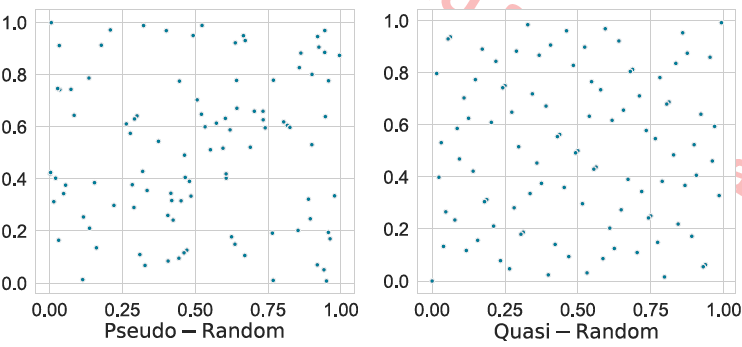
\includegraphics[width=0.7\linewidth]{FileAusiliari/Screenshots/Figure9-3.png}
    \caption{均勻分佈生成的 pseudo-random 變數與 quasi-random 變數的比較。}
    \label{fig:random}
\end{figure}

\term{rocRAND} 提供了生成 quasi-random 變數所需的 API。\lstref{lst:quasi} 中展示了一個範例。這些 API 與生成 pseudo-random 變數的 API 類似,但在創建 quasi-random 變數生成器時有所不同,因為需要使用 \term{ROCRAND\_RNG\_QUASI\_DEFAULT}。此外,還必須指定隨機變量的維度。如果維度為 2,隨機生成器將生成一組由兩個隨機數組成的數據,分別作為 x 軸和 y 軸的值,以便充分填滿空間。

\begin{lstlisting}[language=C, caption={一個生成 100 萬個 pseudo-random 變數的 \term{rocRAND} 函式。}, captionpos=t, label={lst:quasi}]
#include <hip∕hip_runtime.h>
#include <rocrand.h>
#include <stdio.h>
#include <time.h>

int main() {
    size_t n = 1048576;

    rocrand_generator gen;
    float *d_rand;

    h_rand = (float *)malloc(sizeof(float) * n);
    hipMalloc((void **)&d_rand, n * sizeof(float));

    rocrand_create_generator(&gen, ROCRAND_RNG_QUASI_DEFAULT);
    rocrand_set_quasi_random_generator_dimensions(gen, 2)
    rocrand_set_seed(gen, time(NULL));
    rocrand_generate_uniform(gen, d_rand, n);

    ∕∕ Use the generated random numbers.

    rocrand_destroy_generator(gen);
    hipFree(d_rand);
    return 0;
}
\end{lstlisting}

最後,\term{rocRAND} 函式庫附帶了一個相關的 \term{hipRAND} 函式庫。這兩者被設計為可與 \term{rocBLAS} 和 \term{hipBLAS} 互操作。\term{hipRAND} 函式庫是一個輕量級的相容層,在 AMD 平台上支援 \term{rocRAND},在 NVIDIA 平台上支援 \term{cuRAND}。\term{hipRAND} 函式庫的 API 與 \term{rocBLAS} 的結構相似,因此本章將省略對 \term{hipRAND} 的詳細介紹。

\section{結語}
在本章中,我們展示了幾個 \term{ROCm} 函式庫的功能,包括 \term{rocBLAS}、\term{rocSPARSE}、\term{rocFFT} 和 \term{rocRAND}。這些函式庫為程式設計師提供了一種簡單且高效的機制,使其能夠在應用程式中充分利用 GPU 的運算能力。我們仍然建議剛開始學習 HIP 程式設計的初學者自行撰寫 kernel。當開發人員開始處理更複雜的應用程式時,這些函式庫的可用性在許多情況下提供了一種高效且高性能的解決方案。
我們甚至鼓勵程式設計師對自己手寫的演算法進行效能分析,並將其效能與 \term{ROCm} 函式庫對相同演算法的實現進行比較。程式設計師可以撰寫一個矩陣乘法 kernel,然後將其程式碼與 \term{rocBLAS} 函式庫提供的矩陣乘法操作進行比較。這對程式設計師來說是一個很好的學習機會。在分析兩種實現之間的效能差異後,程式設計師可以利用這些新知識來提升未來 HIP 程式的效率。